% !TeX spellcheck = en_GB
\section{Theoretical Background}
In the following some physical concepts needed for the understanding of this experiment are explained.
%\subsection{Physical Concepts}
\subsection{Colour Centres}




Diamond structure is a well know and stuidies in crystalography, It lattice consist in a cubic structure based on 8 Carbon atoms, two tetrahedrally bonded atoms in each primitive. The diamond lattice is basically two face-centered cubic lattices, being the face centeres (FCC) atom on one cell the vertice of the other. Since there are two  identical atoms per unit cell, there is no Absortion of photon in the IR-region, This mean that a purediamond can not have fluorecence properties (in first order) but this propertie can be achive with changes due impurities in the structure. This properties are call Colour centers.

Colour centres (CC) are a kind of point defects in crystal structures which contain a electron that absorbs light of certain wavelengths. This basic defect in the regular spacing of atoms within a solid that absorbs visible light of a particular colour, lending a characteristic colour to the solid. \\

There are more then 100 luminescent defects in diamond. another name that is knowsn is F-centre (German Farbe, “colour”), results from the absence of a negatively charged ion from a particular point in an ionic solid. This vacancy, which acts like a positively charged particle, attracts and traps an electron, and their combination constitutes an Colour-centre.  One of the most abundant and also  studied one is the  Nitrogen related defects, or Nitrogen-Vacancy centeres (NV) , because  nitrogen is a prominent impurity in the material, In next section we will talk in more detail about its oproperties.


\subsection{NV-Centres in Diamonds}
\label{sec:nvcentres}
 The NV-centes are a defect or imurity in the diamond structure, where two carbon atom in the secondary fcc are replaced , one by a nitrogen atom and the second one by a  vacant. The single substitutional nitrogen has an infrared mode of vibration. Nitrogen aggregates are, pairs of neighbouring substitutional atoms, the nitrogen aggregates, and it neibours that leed to different combination ( eigthin total usually labelled according to corresponding Miller indices) in the laticies that have distinct infrared spectra. In the next figure, the Fist Fcc latice of the diamond is shown and in the ceond structure one of the carbons was reaplced by the $N$. NV-center can exist in two charge states, the neutral $NV^{0}$ state and the negatively charged $NV^{-}$ state that have diferent energy levels and alloud transition.
 
The most interenting properties of the NV centers is its absortion and emission fluorecence at red region, properti fundamentalthat will be studied in this experiment, and is mostly due to physical effects by the magnetic moment. A simplified quantum structure of the NV center can be seen in the fig .... where the ground stade and exited stade are contructed by triplet stades with a distance of 1.945 eV in between, here calles $^{3}A_{2}$ and $^{3}E$  respectivelly. The main radiative connection between the ground state and the excited state is due to the zero phonon line (ZPL). For the negatively charged NV center, this transition contributes to a wavelength of $\lambda_{zpl} = 637\,\mathrm{nm}$ and has a lifetime of 10-30 ns.(To observe the ZPL, a simple absortion emition proces was done with a 519nm laser was done, identifin this peak at... .) 
An aditional proces from the exited stade is a nonradiative emission into the metastable singlet state $\left|s\right\rangle$ . This can either occur from the state $\left| e,ms\right\rangle$, in a weak non-radiative decay.

\begin{figure}
	\centering
	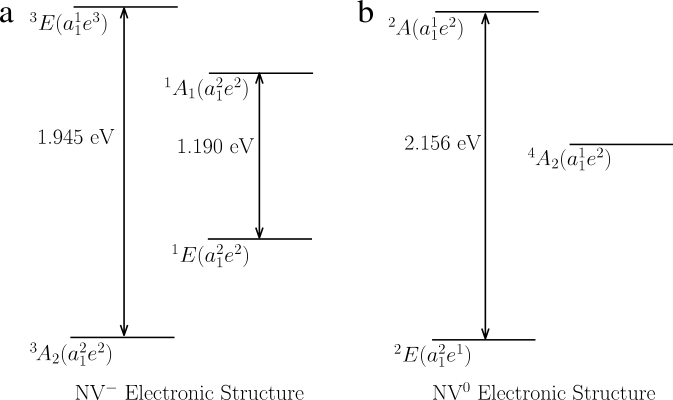
\includegraphics[width=0.5\textwidth]{../figures/nv-centre.png}
	\caption{Electronic structure of (a) NV$^-$ and (b) NV$^0$ centres \cite{doherty}}
	\label{fig:nvcentres}
\end{figure}


%\subsection{Experimental Methods}
\subsection{Optically Detected Magnetic Resonance}







